
\section{Knowing what Git is and what GitHub is}
\label{SectionSSHGit}

If you've already got familiar with Git, then you could skip this task.

If you have been working with CVS (Concurrent Versions System, not the CVS
store), SVN (Subversion), or Mercurial, then Git is yet another revision control
tool, which has some unique features. If you don't have any exprience in working
with a revision control system, then probably you might want to first learn what
a \emph{revision control} system is.

\begin{quote}
\emph{Revision control, also known as version control and source control (and
an aspect of software configuration management), is the management of changes
to documents, computer programs, large web sites, and other collections of
information.}\footnote{\url{http://en.wikipedia.org/wiki/Revision_control}}
\end{quote}

In general, revision control is super useful in software engineering.
Intuitively, let us think about two use cases of revision control:

\begin{enumerate}

\item After days of development, you realized that you reached a dead-end and
wanted to revert back to a very early version, but you couldn't remember what
those changes you made during those days are, even though you might have your
projects backed up and marked by dates. A revision control system could help you
manage the changes you made each time you submit your change.

\item Your friend admitted to work with you on your project, and you two are
writing different parts of the project at the same time. Once you two decided to
merge your parts, you found that you both had modified the same file, and you
had to manually (or with some extra tool) check the difference between your
modifications. A revision control system could automatically merge the changes
you made.

\end{enumerate}

From Wikipedia, Git\footnote{\url{http://git-scm.com}} is described as \emph{a
distributed revision control and source code management (SCM) system with an
emphasis on speed.} Besides the consideration of speed, you can find other
features, e.g., \emph{distributed development}, \emph{non-linear development},
etc., at \url{http://git-scm.com/about}. Note that the entry page just
introduces the first of many features, and you need to click on the other
circles to view the other features. We recommend you to read at least the
feature description page and the Wikipedia page to know those basic concepts of
Git, and you might also want to further read the Pro Git
book\footnote{\url{http://git-scm.com/book}} to know it better.

In addition, you should have an idea of the following concepts in Git, which are
the most important ones for our course.

\begin{center}
\textbf{commit, index, branch}
\end{center}

\noindent and you should also be familiar with the following commands:

\begin{center}
\texttt{add, ignore, commit, fetch, pull, push, branch}
\end{center}

In this homework, we will show you how to run Git commands with EGit (the Git
plug-in for Eclipse), and especially demonstrate the usages of \texttt{commit}
and \texttt{push}. You are going to use more of them in your next few homeworks.

Finally, GitHub is a web-based hosting service for software development projects
that use the Git revision control
system.\footnote{\url{https://en.wikipedia.org/wiki/GitHub}} What you might want
to add to your Bookmarks (or Favorates, or other social bookmark site) is the
help page (\url{http://help.github.com/}).

\section{Creating your account on GitHub}

\begin{figure}[t]
\centering
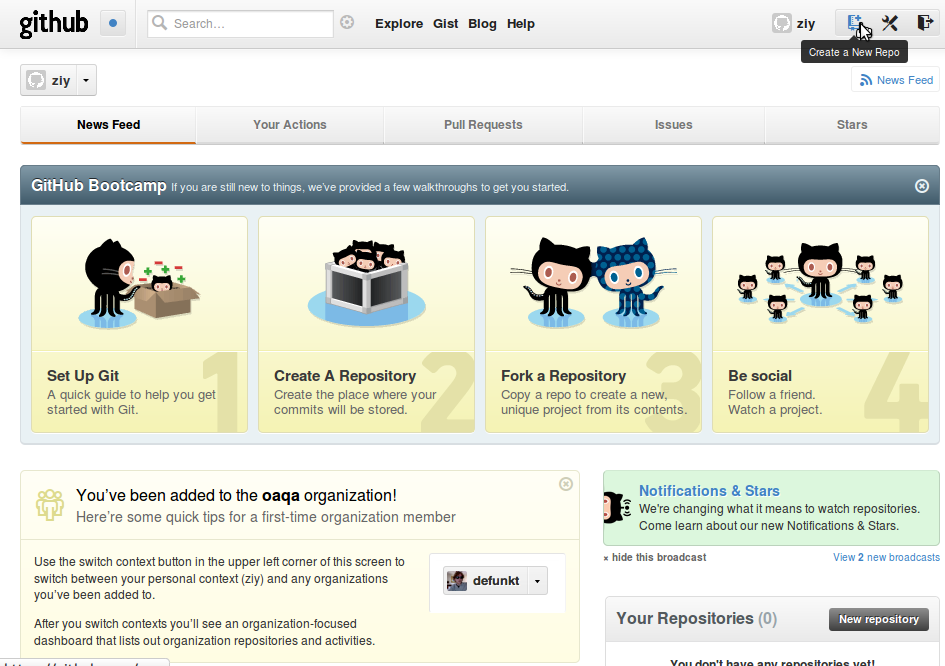
\includegraphics[scale=0.3]{git-01-register}
\caption{Registering a GitHub account\label{git-01-register}}
\end{figure}

In this task, you are required to register an account at GitHub and create a
public repository.

\begin{qa}

\item[Q1] Is there any difference between a public and a private repository?

\item[A1] Every piece of code in a public repository can be seen by everyone
from everywhere in the world even if he/she doesn't have a GitHub account. Codes
in private repositories can be seen by the owner and the collaborators only.

\item[Q2] You asked us to create a public repository for homework codebase. But
I feel it uncomfortable that other students might ``plagiarize'' my code and use
for their homework submission.

\item[A2] For Homework 0, you will soon realize all the codes will have been
available in this guideline. If you prefer to fork other's project to make your
project, then you must already be an expert. For the rest of the homeworks, we
believe if someone ``plagiarizes'' your codebase, know what is going on in your
project, implement his/her code to work best with your code, and eventually
achieve the best performance, then why not to let others look at your code?

\end{qa}

\begin{enumerate}

\item Registration is easy, but you will need to generate an SSH key and add
that to your GitHub account. This is a platform specific task, and we suggest
you to refer to the help page at
\url{http://help.github.com/articles/generating-ssh-keys}. Note that if you are
using a Windows machine, you will need a Git Bash to run the commands, and it
would be better not using a passphrase when generating the public key (instead
directly pressing \textbf{Enter}), or the project will stuck at release because
Eclipse is waiting for a passphrase but it doesn't prompt us to do
that.\footnote{Reported by Hector Liu.} Another important step is to ensure you
have verified your email address on GitHub, otherwise there might be risk that
when Maven is executing ``git push'' command, it will also hang forever.

\begin{qa}

\item[Q1] What is SSH? What is a public key? Why do I need that?

\item[A1] Informally, SSH allows you to securely connect to a remote server.
Still informally, a public key allows you to make a connection without typing
your password over and over again, but the server can still identify the person
who tries to log in isn't anybody else but you! Because a Maven plug-in will
execute Git commands without bothering you to type your passwords, GitHub needs
to know your public key. If you are really interested in public-key
cryptography, you need to find a textbook to read, which is far far beyond the
scope of our course.

\end{qa}

\item Creating a repository is also easy, on the top-right corner of the
homepage, you will find an icon to create a repository. See Figure
\ref{git-01-register}.

\item Type in a name for the repository. For example as shown in Figure
\ref{git-02-create-repo}, we suggest to name it as \texttt{hw0-ANDREWID}. 
%Note that the repository name should be unique in all the GitHub repositories of all
%users, which means there is a chance the name might already be taken by someone
%else. But don't worry. 
Note, however, that the repository name can be different from your Java
project name and Maven artifact name (which will become the name of your
submission). 
%So just go ahead for a different name.

\begin{figure}[t]
\centering
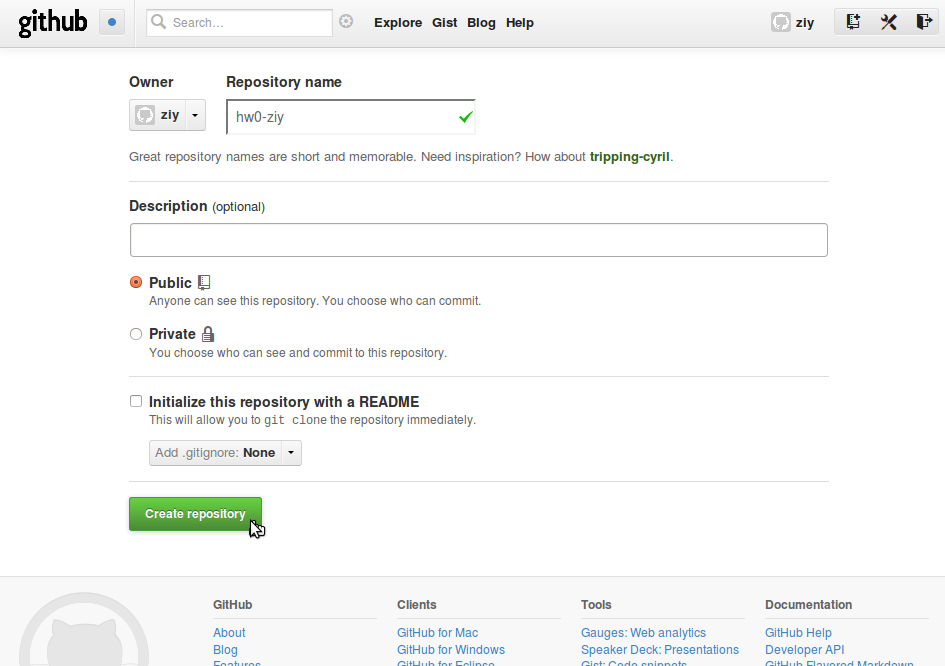
\includegraphics[scale=0.3]{git-02-create-repo}
\caption{Creating a public repository\label{git-02-create-repo}}
\end{figure}

\begin{figure}[t]
\centering
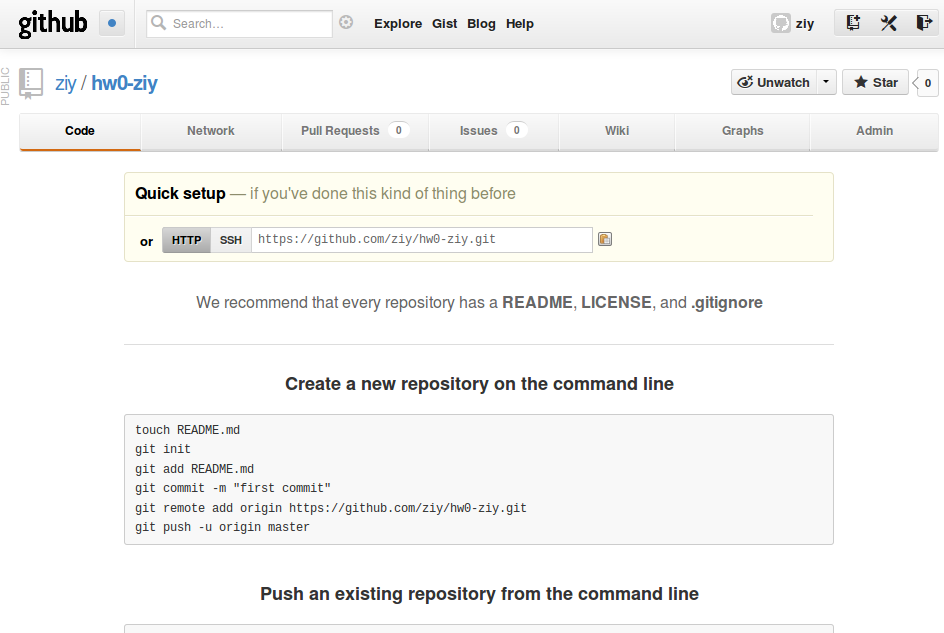
\includegraphics[scale=0.3]{git-03-uri}
\caption{Copying your repository URI\label{git-03-uri}}
\end{figure}

\item In the end, you will be notified about your repository URI. Copy it, which
is useful in the next step.

\end{enumerate}

